\chapter{Directed graphs}

In this chapter, we focus on two classes of directed graphs:

\begin{itemize}
\item \key{Acyclic graph}:
There are no cycles in the graph,
so there is no path from any node to itself.
\item \key{Successor graph}:
The outdegree of each node is 1,
so each node has a unique successor.
\end{itemize}
It turns out that in both cases,
we can design efficient algorithms that are based
on the special properties of the graphs.

\section{Topological sorting}

\index{topological sorting}
\index{cycle}

A \key{topological sort} is a ordering
of the nodes of a directed graph
where node $a$ is always before node $b$
if there is a path from node $a$ to node $b$.
For example, for the graph
\begin{center}
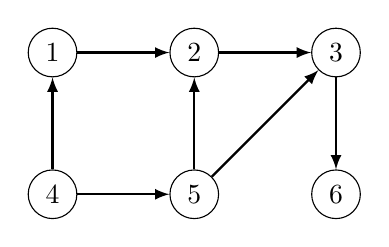
\begin{tikzpicture}[scale=0.9]
\node[draw, circle] (1) at (1,5) {$1$};
\node[draw, circle] (2) at (3,5) {$2$};
\node[draw, circle] (3) at (5,5) {$3$};
\node[draw, circle] (4) at (1,3) {$4$};
\node[draw, circle] (5) at (3,3) {$5$};
\node[draw, circle] (6) at (5,3) {$6$};

\path[draw,thick,->,>=latex] (1) -- (2);
\path[draw,thick,->,>=latex] (2) -- (3);
\path[draw,thick,->,>=latex] (4) -- (1);
\path[draw,thick,->,>=latex] (4) -- (5);
\path[draw,thick,->,>=latex] (5) -- (2);
\path[draw,thick,->,>=latex] (5) -- (3);
\path[draw,thick,->,>=latex] (3) -- (6);
\end{tikzpicture}
\end{center}
a possible topological sort is
$[4,1,5,2,3,6]$:
\begin{center}
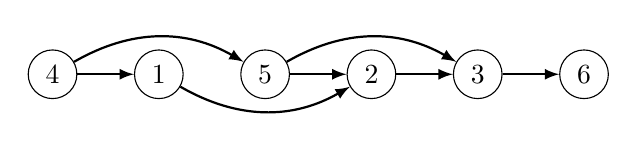
\begin{tikzpicture}[scale=0.9]
\node[draw, circle] (1) at (-6,0) {$1$};
\node[draw, circle] (2) at (-3,0) {$2$};
\node[draw, circle] (3) at (-1.5,0) {$3$};
\node[draw, circle] (4) at (-7.5,0) {$4$};
\node[draw, circle] (5) at (-4.5,0) {$5$};
\node[draw, circle] (6) at (-0,0) {$6$};

\path[draw,thick,->,>=latex] (1) edge [bend right=30] (2);
\path[draw,thick,->,>=latex] (2) -- (3);
\path[draw,thick,->,>=latex] (4) -- (1);
\path[draw,thick,->,>=latex] (4) edge [bend left=30] (5);
\path[draw,thick,->,>=latex] (5) -- (2);
\path[draw,thick,->,>=latex] (5) edge [bend left=30]  (3);
\path[draw,thick,->,>=latex] (3) -- (6);
\end{tikzpicture}
\end{center}

A topological sort always exists
if the graph is acyclic.
However, if the graph contains a cycle,
it is not possible to find a topological sort
because no node in the cycle can appear
before other nodes in the cycle in the ordering.
It turns out that we can use depth-first search
to both construct a topological sort or find out
that it is not possible because the graph contains a cycle.

\subsubsection{Algorithm}

The idea is to go through the nodes in the graph
and always begin a depth-first search if the
node has not been processed yet.
During each search, the nodes have three possible states:

\begin{itemize}
\item state 0: the node has not been processed (white)
\item state 1: the node is under processing (light gray)
\item state 2: the node has been processed (dark gray)
\end{itemize}

Initially, the state of each node is 0.
When a search reaches a node for the first time,
the state of the node becomes 1.
Finally, after all neighbors of a node have
been processed, the state of the node becomes 2.

If the graph contains a cycle, we will realize this
during the search because sooner or later
we will arrive at a node whose state is 1.
In this case, it is not possible to construct a topological sort.

If the graph doesn't contain a cycle, we can construct
a topological sort by adding each node to the end of a list
when its state becomes 2.
This list in reverse order is a topological sort.

\subsubsection{Example 1}

In the example graph, the search first proceeds
from node 1 to node 6:

\begin{center}
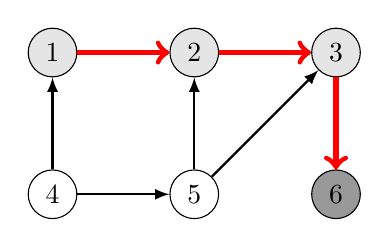
\begin{tikzpicture}[scale=0.9]
\node[draw, circle,fill=gray!20] (1) at (1,5) {$1$};
\node[draw, circle,fill=gray!20] (2) at (3,5) {$2$};
\node[draw, circle,fill=gray!20] (3) at (5,5) {$3$};
\node[draw, circle] (4) at (1,3) {$4$};
\node[draw, circle] (5) at (3,3) {$5$};
\node[draw, circle,fill=gray!80] (6) at (5,3) {$6$};

\path[draw,thick,->,>=latex] (4) -- (1);
\path[draw,thick,->,>=latex] (4) -- (5);
\path[draw,thick,->,>=latex] (5) -- (2);
\path[draw,thick,->,>=latex] (5) -- (3);
%\path[draw,thick,->,>=latex] (3) -- (6);

\path[draw=red,thick,->,line width=2pt] (1) -- (2);
\path[draw=red,thick,->,line width=2pt] (2) -- (3);
\path[draw=red,thick,->,line width=2pt] (3) -- (6);
\end{tikzpicture}
\end{center}

Now node 6 has been processed, so it is added to the list.
After this, the search returns back:

\begin{center}
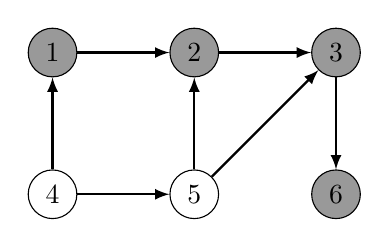
\begin{tikzpicture}[scale=0.9]
\node[draw, circle,fill=gray!80] (1) at (1,5) {$1$};
\node[draw, circle,fill=gray!80] (2) at (3,5) {$2$};
\node[draw, circle,fill=gray!80] (3) at (5,5) {$3$};
\node[draw, circle] (4) at (1,3) {$4$};
\node[draw, circle] (5) at (3,3) {$5$};
\node[draw, circle,fill=gray!80] (6) at (5,3) {$6$};

\path[draw,thick,->,>=latex] (1) -- (2);
\path[draw,thick,->,>=latex] (2) -- (3);
\path[draw,thick,->,>=latex] (4) -- (1);
\path[draw,thick,->,>=latex] (4) -- (5);
\path[draw,thick,->,>=latex] (5) -- (2);
\path[draw,thick,->,>=latex] (5) -- (3);
\path[draw,thick,->,>=latex] (3) -- (6);
\end{tikzpicture}
\end{center}

At this point, the list contains values $[6,3,2,1]$.
The next search begins at node 4:

\begin{center}
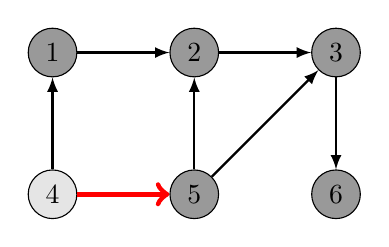
\begin{tikzpicture}[scale=0.9]
\node[draw, circle,fill=gray!80] (1) at (1,5) {$1$};
\node[draw, circle,fill=gray!80] (2) at (3,5) {$2$};
\node[draw, circle,fill=gray!80] (3) at (5,5) {$3$};
\node[draw, circle,fill=gray!20] (4) at (1,3) {$4$};
\node[draw, circle,fill=gray!80] (5) at (3,3) {$5$};
\node[draw, circle,fill=gray!80] (6) at (5,3) {$6$};

\path[draw,thick,->,>=latex] (1) -- (2);
\path[draw,thick,->,>=latex] (2) -- (3);
\path[draw,thick,->,>=latex] (4) -- (1);
%\path[draw,thick,->,>=latex] (4) -- (5);
\path[draw,thick,->,>=latex] (5) -- (2);
\path[draw,thick,->,>=latex] (5) -- (3);
\path[draw,thick,->,>=latex] (3) -- (6);

\path[draw=red,thick,->,line width=2pt] (4) -- (5);
\end{tikzpicture}
\end{center}

Thus, the final list is $[6,3,2,1,5,4]$.
We have processed all nodes, so a topological sort has
been found.
The topological sort is the reverse list
$[4,5,1,2,3,6]$:

\begin{center}
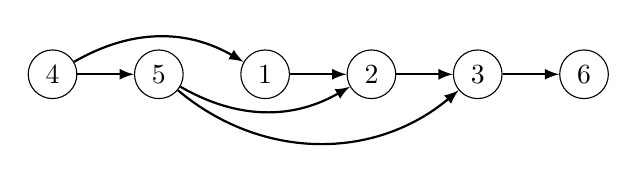
\begin{tikzpicture}[scale=0.9]
\node[draw, circle] (1) at (3,0) {$1$};
\node[draw, circle] (2) at (4.5,0) {$2$};
\node[draw, circle] (3) at (6,0) {$3$};
\node[draw, circle] (4) at (0,0) {$4$};
\node[draw, circle] (5) at (1.5,0) {$5$};
\node[draw, circle] (6) at (7.5,0) {$6$};

\path[draw,thick,->,>=latex] (1) -- (2);
\path[draw,thick,->,>=latex] (2) -- (3);
\path[draw,thick,->,>=latex] (4) edge [bend left=30] (1);
\path[draw,thick,->,>=latex] (4) -- (5);
\path[draw,thick,->,>=latex] (5) edge [bend right=30] (2);
\path[draw,thick,->,>=latex] (5) edge [bend right=40] (3);
\path[draw,thick,->,>=latex] (3) -- (6);
\end{tikzpicture}
\end{center}

Note that a topological sort is not unique,
but there can be several topological sorts for a graph.

\subsubsection{Example 2}

Let's consider another example where we can't
construct a topological sort because there is a
cycle in the graph:

\begin{center}
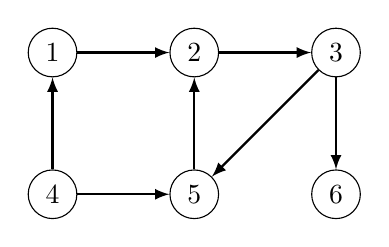
\begin{tikzpicture}[scale=0.9]
\node[draw, circle] (1) at (1,5) {$1$};
\node[draw, circle] (2) at (3,5) {$2$};
\node[draw, circle] (3) at (5,5) {$3$};
\node[draw, circle] (4) at (1,3) {$4$};
\node[draw, circle] (5) at (3,3) {$5$};
\node[draw, circle] (6) at (5,3) {$6$};

\path[draw,thick,->,>=latex] (1) -- (2);
\path[draw,thick,->,>=latex] (2) -- (3);
\path[draw,thick,->,>=latex] (4) -- (1);
\path[draw,thick,->,>=latex] (4) -- (5);
\path[draw,thick,->,>=latex] (5) -- (2);
\path[draw,thick,->,>=latex] (3) -- (5);
\path[draw,thick,->,>=latex] (3) -- (6);
\end{tikzpicture}
\end{center}
Now the search proceeds as follows:
\begin{center}
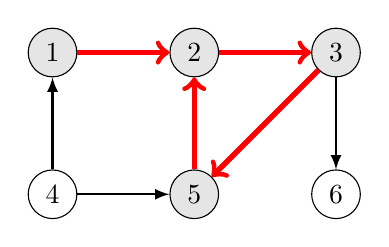
\begin{tikzpicture}[scale=0.9]
\node[draw, circle,fill=gray!20] (1) at (1,5) {$1$};
\node[draw, circle,fill=gray!20] (2) at (3,5) {$2$};
\node[draw, circle,fill=gray!20] (3) at (5,5) {$3$};
\node[draw, circle] (4) at (1,3) {$4$};
\node[draw, circle,fill=gray!20] (5) at (3,3) {$5$};
\node[draw, circle] (6) at (5,3) {$6$};

\path[draw,thick,->,>=latex] (4) -- (1);
\path[draw,thick,->,>=latex] (4) -- (5);
\path[draw,thick,->,>=latex] (3) -- (6);

\path[draw=red,thick,->,line width=2pt] (1) -- (2);
\path[draw=red,thick,->,line width=2pt] (2) -- (3);
\path[draw=red,thick,->,line width=2pt] (3) -- (5);
\path[draw=red,thick,->,line width=2pt] (5) -- (2);
\end{tikzpicture}
\end{center}
The search reaches node 2 whose state is 1
which means the graph contains a cycle.
In this case, the cycle is $2 \rightarrow 3 \rightarrow 5 \rightarrow 2$.

\section{Dynamic programming}

If a directed graph is acyclic,
dynamic programming can be applied to it.
For example, we can solve the following
problems concerning paths from a starting node
to an ending node efficiently in $O(n+m)$ time:

\begin{itemize}
\item how many different paths are there?
\item what is the shortest/longest path?
\item what is the minimum/maximum number of edges in a path?
\item which nodes certainly appear in the path?
\end{itemize}

\subsubsection{Counting the number of paths}

As an example, let's calculate the number of paths
from a starting node to an ending node
in a directed, acyclic graph.
For example, in the graph

\begin{center}
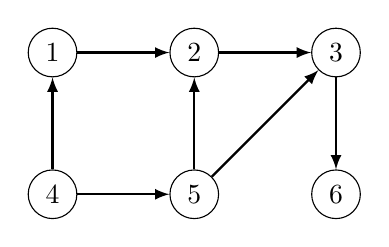
\begin{tikzpicture}[scale=0.9]
\node[draw, circle] (1) at (1,5) {$1$};
\node[draw, circle] (2) at (3,5) {$2$};
\node[draw, circle] (3) at (5,5) {$3$};
\node[draw, circle] (4) at (1,3) {$4$};
\node[draw, circle] (5) at (3,3) {$5$};
\node[draw, circle] (6) at (5,3) {$6$};

\path[draw,thick,->,>=latex] (1) -- (2);
\path[draw,thick,->,>=latex] (2) -- (3);
\path[draw,thick,->,>=latex] (4) -- (1);
\path[draw,thick,->,>=latex] (4) -- (5);
\path[draw,thick,->,>=latex] (5) -- (2);
\path[draw,thick,->,>=latex] (5) -- (3);
\path[draw,thick,->,>=latex] (3) -- (6);
\end{tikzpicture}
\end{center}
there are 3 paths from node 4 to node 6:
\begin{itemize}
\item $4 \rightarrow 1 \rightarrow 2 \rightarrow 3 \rightarrow 6$
\item $4 \rightarrow 5 \rightarrow 2 \rightarrow 3 \rightarrow 6$
\item $4 \rightarrow 5 \rightarrow 3 \rightarrow 6$
\end{itemize}
The idea is to go through the nodes in a topological sort,
and calculate for each node the total number of paths
that reach the node from different directions.
In this case, the topological sort is as follows:

\begin{center}
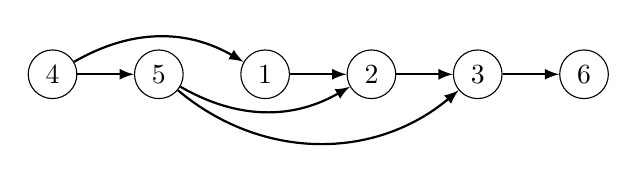
\begin{tikzpicture}[scale=0.9]
\node[draw, circle] (1) at (3,0) {$1$};
\node[draw, circle] (2) at (4.5,0) {$2$};
\node[draw, circle] (3) at (6,0) {$3$};
\node[draw, circle] (4) at (0,0) {$4$};
\node[draw, circle] (5) at (1.5,0) {$5$};
\node[draw, circle] (6) at (7.5,0) {$6$};

\path[draw,thick,->,>=latex] (1) -- (2);
\path[draw,thick,->,>=latex] (2) -- (3);
\path[draw,thick,->,>=latex] (4) edge [bend left=30] (1);
\path[draw,thick,->,>=latex] (4) -- (5);
\path[draw,thick,->,>=latex] (5) edge [bend right=30] (2);
\path[draw,thick,->,>=latex] (5) edge [bend right=40] (3);
\path[draw,thick,->,>=latex] (3) -- (6);
\end{tikzpicture}
\end{center}
The numbers of paths are as follows:

\begin{center}
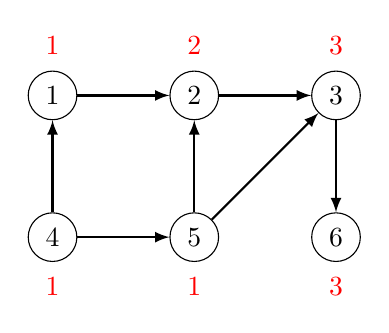
\begin{tikzpicture}[scale=0.9]
\node[draw, circle] (1) at (1,5) {$1$};
\node[draw, circle] (2) at (3,5) {$2$};
\node[draw, circle] (3) at (5,5) {$3$};
\node[draw, circle] (4) at (1,3) {$4$};
\node[draw, circle] (5) at (3,3) {$5$};
\node[draw, circle] (6) at (5,3) {$6$};

\path[draw,thick,->,>=latex] (1) -- (2);
\path[draw,thick,->,>=latex] (2) -- (3);
\path[draw,thick,->,>=latex] (4) -- (1);
\path[draw,thick,->,>=latex] (4) -- (5);
\path[draw,thick,->,>=latex] (5) -- (2);
\path[draw,thick,->,>=latex] (5) -- (3);
\path[draw,thick,->,>=latex] (3) -- (6);

\node[color=red] at (1,2.3) {$1$};
\node[color=red] at (3,2.3) {$1$};
\node[color=red] at (5,2.3) {$3$};
\node[color=red] at (1,5.7) {$1$};
\node[color=red] at (3,5.7) {$2$};
\node[color=red] at (5,5.7) {$3$};
\end{tikzpicture}
\end{center}

For example, there is an edge to node 2 from nodes 1 and 5.
There is one path from node 4 to both node 1 and 5,
so there are two paths from node 4 to node 2.
Correspondingly, there is an edge to node 3 from nodes 2 and 5
that correspond to two and one paths from node 4.

\subsubsection{Extending Dijkstra's algorithm}

\index{Dijkstra's algorithm}

A by-product of Dijkstra's algorithm is a directed, acyclic
graph that shows for each node in the original graph
the possible ways to reach the node using a shortest path
from the starting node.
Dynamic programming can be applied also to this graph.
For example, in the graph
\begin{center}
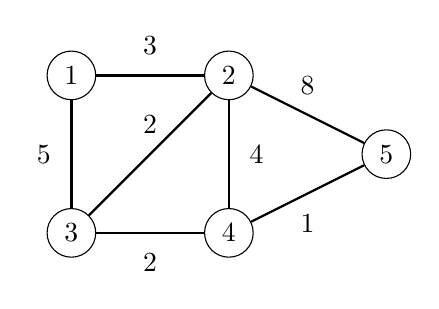
\begin{tikzpicture}
\node[draw, circle] (1) at (0,0) {$1$};
\node[draw, circle] (2) at (2,0) {$2$};
\node[draw, circle] (3) at (0,-2) {$3$};
\node[draw, circle] (4) at (2,-2) {$4$};
\node[draw, circle] (5) at (4,-1) {$5$};

\path[draw,thick,-] (1) -- node[font=\small,label=above:3] {} (2);
\path[draw,thick,-] (1) -- node[font=\small,label=left:5] {} (3);
\path[draw,thick,-] (2) -- node[font=\small,label=right:4] {} (4);
\path[draw,thick,-] (2) -- node[font=\small,label=above:8] {} (5);
\path[draw,thick,-] (3) -- node[font=\small,label=below:2] {} (4);
\path[draw,thick,-] (4) -- node[font=\small,label=below:1] {} (5);
\path[draw,thick,-] (2) -- node[font=\small,label=above:2] {} (3);
\end{tikzpicture}
\end{center}
the following edges can belong to the shortest paths
from node 1:
\begin{center}
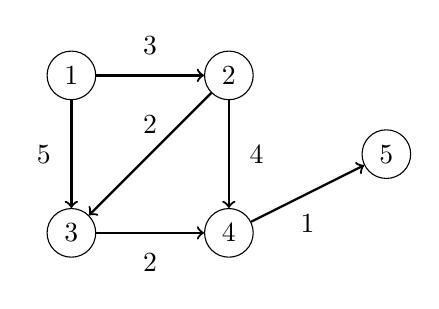
\begin{tikzpicture}
\node[draw, circle] (1) at (0,0) {$1$};
\node[draw, circle] (2) at (2,0) {$2$};
\node[draw, circle] (3) at (0,-2) {$3$};
\node[draw, circle] (4) at (2,-2) {$4$};
\node[draw, circle] (5) at (4,-1) {$5$};

\path[draw,thick,->] (1) -- node[font=\small,label=above:3] {} (2);
\path[draw,thick,->] (1) -- node[font=\small,label=left:5] {} (3);
\path[draw,thick,->] (2) -- node[font=\small,label=right:4] {} (4);
\path[draw,thick,->] (3) -- node[font=\small,label=below:2] {} (4);
\path[draw,thick,->] (4) -- node[font=\small,label=below:1] {} (5);
\path[draw,thick,->] (2) -- node[font=\small,label=above:2] {} (3);
\end{tikzpicture}
\end{center}

Now we can, for example, calculate the number of
shortest paths from node 1 to node 5
using dynamic programming:
\begin{center}
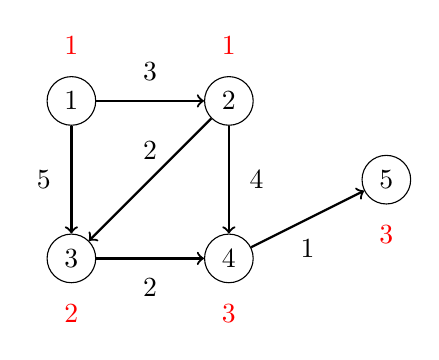
\begin{tikzpicture}
\node[draw, circle] (1) at (0,0) {$1$};
\node[draw, circle] (2) at (2,0) {$2$};
\node[draw, circle] (3) at (0,-2) {$3$};
\node[draw, circle] (4) at (2,-2) {$4$};
\node[draw, circle] (5) at (4,-1) {$5$};

\path[draw,thick,->] (1) -- node[font=\small,label=above:3] {} (2);
\path[draw,thick,->] (1) -- node[font=\small,label=left:5] {} (3);
\path[draw,thick,->] (2) -- node[font=\small,label=right:4] {} (4);
\path[draw,thick,->] (3) -- node[font=\small,label=below:2] {} (4);
\path[draw,thick,->] (4) -- node[font=\small,label=below:1] {} (5);
\path[draw,thick,->] (2) -- node[font=\small,label=above:2] {} (3);

\node[color=red] at (0,0.7) {$1$};
\node[color=red] at (2,0.7) {$1$};
\node[color=red] at (0,-2.7) {$2$};
\node[color=red] at (2,-2.7) {$3$};
\node[color=red] at (4,-1.7) {$3$};
\end{tikzpicture}
\end{center}

\subsubsection{Representing problems as graphs}

Actually, any dynamic programming problem
can be represented as a directed, acyclic graph.
In such a graph, each node is a dynamic programming state,
and the edges indicate how the states depend on each other.

As an example, consider the problem
where our task is to form a sum of money $x$
using coins
$\{c_1,c_2,\ldots,c_k\}$.
In this case, we can construct a graph where
each node corresponds to a sum of money,
and the edges show how we can choose coins.
For example, for coins $\{1,3,4\}$ and $x=6$,
the graph is as follows:
\begin{center}
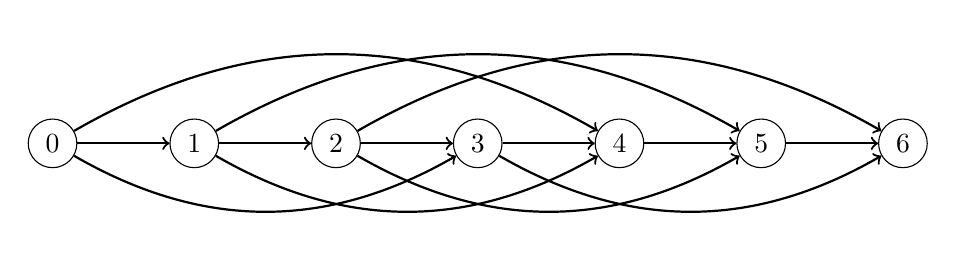
\begin{tikzpicture}[scale=0.9]
\node[draw, circle] (0) at (0,0) {$0$};
\node[draw, circle] (1) at (2,0) {$1$};
\node[draw, circle] (2) at (4,0) {$2$};
\node[draw, circle] (3) at (6,0) {$3$};
\node[draw, circle] (4) at (8,0) {$4$};
\node[draw, circle] (5) at (10,0) {$5$};
\node[draw, circle] (6) at (12,0) {$6$};

\path[draw,thick,->] (0) -- (1);
\path[draw,thick,->] (1) -- (2);
\path[draw,thick,->] (2) -- (3);
\path[draw,thick,->] (3) -- (4);
\path[draw,thick,->] (4) -- (5);
\path[draw,thick,->] (5) -- (6);

\path[draw,thick,->] (0) edge [bend right=30] (3);
\path[draw,thick,->] (1) edge [bend right=30] (4);
\path[draw,thick,->] (2) edge [bend right=30] (5);
\path[draw,thick,->] (3) edge [bend right=30] (6);

\path[draw,thick,->] (0) edge [bend left=30] (4);
\path[draw,thick,->] (1) edge [bend left=30] (5);
\path[draw,thick,->] (2) edge [bend left=30] (6);
\end{tikzpicture}
\end{center}

Using this representation,
the shortest path from node 0 to node $x$
corresponds to a solution with minimum number of coins,
and the total number of paths from node 0 to node $x$
equals the total number of solutions.

\section{Tehokas eteneminen}

\index{seuraajaverkko@seuraajaverkko}
\index{funktionaalinen verkko@funktionaalinen verkko}

Seuraavaksi oletamme, että
suunnaton verkko on \key{seuraajaverkko},
jolloin jokaisen solmun lähtöaste on 1
eli siitä lähtee tasan yksi kaari ulospäin.
Niinpä verkko muodostuu yhdestä tai useammasta
komponentista, joista jokaisessa on yksi sykli
ja joukko siihen johtavia polkuja.

Seuraajaverkosta käytetään joskus nimeä
\key{funktionaalinen verkko}.
Tämä johtuu siitä, että jokaista seuraajaverkkoa
vastaa funktio $f$, joka määrittelee verkon kaaret.
Funktion parametrina on verkon solmu ja
se palauttaa solmusta lähtevän kaaren kohdesolmun.

\begin{samepage}
Esimerkiksi funktio
\begin{center}
\begin{tabular}{r|rrrrrrrrr}
$x$ & 1 & 2 & 3 & 4 & 5 & 6 & 7 & 8 & 9 \\
\hline
$f(x)$ & 3 & 5 & 7 & 6 & 2 & 2 & 1 & 6 & 3 \\
\end{tabular}
\end{center}
\end{samepage}
määrittelee seuraavan verkon:
\begin{center}
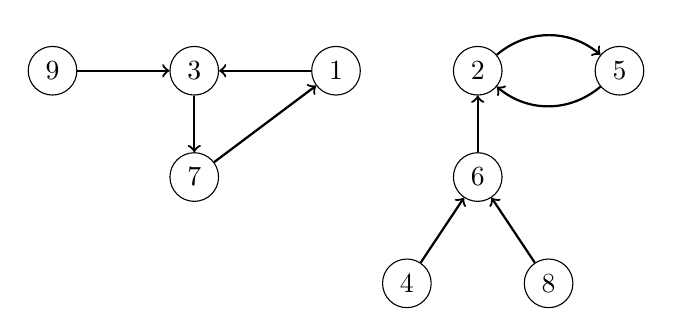
\begin{tikzpicture}[scale=0.9]
\node[draw, circle] (1) at (0,0) {$1$};
\node[draw, circle] (2) at (2,0) {$2$};
\node[draw, circle] (3) at (-2,0) {$3$};
\node[draw, circle] (4) at (1,-3) {$4$};
\node[draw, circle] (5) at (4,0) {$5$};
\node[draw, circle] (6) at (2,-1.5) {$6$};
\node[draw, circle] (7) at (-2,-1.5) {$7$};
\node[draw, circle] (8) at (3,-3) {$8$};
\node[draw, circle] (9) at (-4,0) {$9$};

\path[draw,thick,->] (1) -- (3);
\path[draw,thick,->] (2)  edge [bend left=40] (5);
\path[draw,thick,->] (3) -- (7);
\path[draw,thick,->] (4) -- (6);
\path[draw,thick,->] (5)  edge [bend left=40] (2);
\path[draw,thick,->] (6) -- (2);
\path[draw,thick,->] (7) -- (1);
\path[draw,thick,->] (8) -- (6);
\path[draw,thick,->] (9) -- (3);
\end{tikzpicture}
\end{center}

Koska seuraajaverkon jokaisella solmulla
on yksikäsitteinen seuraaja, voimme määritellä funktion $f(x,k)$,
joka kertoo solmun, johon päätyy solmusta $x$
kulkemalla $k$ askelta.
Esimerkiksi yllä olevassa verkossa $f(4,6)=2$,
koska solmusta 4 päätyy solmuun 2 kulkemalla 6 askelta:

\begin{center}
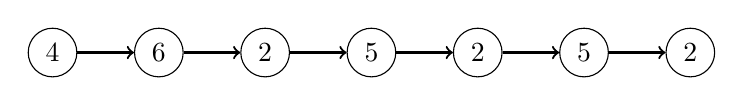
\begin{tikzpicture}[scale=0.9]
\node[draw, circle] (1) at (0,0) {$4$};
\node[draw, circle] (2) at (1.5,0) {$6$};
\node[draw, circle] (3) at (3,0) {$2$};
\node[draw, circle] (4) at (4.5,0) {$5$};
\node[draw, circle] (5) at (6,0) {$2$};
\node[draw, circle] (6) at (7.5,0) {$5$};
\node[draw, circle] (7) at (9,0) {$2$};

\path[draw,thick,->] (1) -- (2);
\path[draw,thick,->] (2) -- (3);
\path[draw,thick,->] (3) -- (4);
\path[draw,thick,->] (4) -- (5);
\path[draw,thick,->] (5) -- (6);
\path[draw,thick,->] (6) -- (7);
\end{tikzpicture}
\end{center}

Suoraviivainen tapa laskea arvo $f(x,k)$
on käydä läpi polku askel askeleelta, mihin kuluu aikaa $O(k)$.
Sopivan esikäsittelyn avulla voimme laskea kuitenkin
minkä tahansa arvon $f(x,k)$ ajassa $O(\log k)$.

Ideana on laskea etukäteen kaikki arvot $f(x,k)$, kun $k$ on 2:n potenssi
ja enintään $u$, missä $u$ on suurin mahdollinen määrä
askeleita, joista olemme kiinnostuneita.
Tämä onnistuu tehokkaasti, koska voimme käyttää rekursiota

\begin{equation*}
    f(x,k) = \begin{cases}
               f(x)              & k = 1\\
               f(f(x,k/2),k/2)   & k > 1\\
           \end{cases}
\end{equation*}

Arvojen $f(x,k)$ esilaskenta vie aikaa $O(n \log u)$,
koska jokaisesta solmusta lasketaan $O(\log u)$ arvoa.
Esimerkin tapauksessa taulukko alkaa muodostua seuraavasti:

\begin{center}
\begin{tabular}{r|rrrrrrrrr}
$x$ & 1 & 2 & 3 & 4 & 5 & 6 & 7 & 8 & 9 \\
\hline
$f(x,1)$ & 3 & 5 & 7 & 6 & 2 & 2 & 1 & 6 & 3 \\
$f(x,2)$ & 7 & 2 & 1 & 2 & 5 & 5 & 3 & 2 & 7 \\
$f(x,4)$ & 3 & 2 & 7 & 2 & 5 & 5 & 1 & 2 & 3 \\
$f(x,8)$ & 7 & 2 & 1 & 2 & 5 & 5 & 3 & 2 & 7 \\
$\cdots$ \\
\end{tabular}
\end{center}

Tämän jälkeen funktion $f(x,k)$ arvon saa laskettua
esittämällä luvun $k$ summana 2:n potensseja.
Esimerkiksi jos haluamme laskea arvon $f(x,11)$,
muodostamme ensin esityksen $11=8+2+1$.
Tämän ansiosta
\[f(x,11)=f(f(f(x,8),2),1).\]
Esimerkiksi yllä olevassa verkossa 
\[f(4,11)=f(f(f(4,8),2),1)=5.\]

Tällaisessa esityksessä on aina
$O(\log k)$ osaa, joten arvon $f(x,k)$ laskemiseen
kuluu aikaa $O(\log k)$.

\section{Syklin tunnistaminen}

\index{sykli@sykli}
\index{syklin tunnistaminen@syklin tunnistaminen}

Kiinnostavia kysymyksiä seuraajaverkossa ovat,
minkä solmun kohdalla saavutaan sykliin
solmusta $x$ lähdettäessä
ja montako solmua kyseiseen sykliin kuuluu.
Esimerkiksi verkossa

\begin{center}
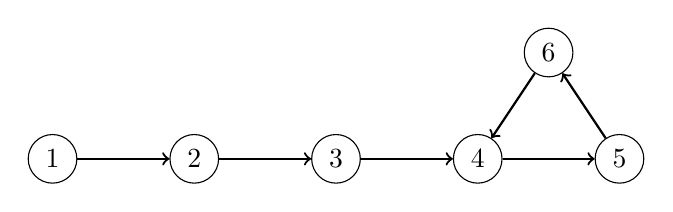
\begin{tikzpicture}[scale=0.9]
\node[draw, circle] (5) at (0,0) {$5$};
\node[draw, circle] (4) at (-2,0) {$4$};
\node[draw, circle] (6) at (-1,1.5) {$6$};
\node[draw, circle] (3) at (-4,0) {$3$};
\node[draw, circle] (2) at (-6,0) {$2$};
\node[draw, circle] (1) at (-8,0) {$1$};

\path[draw,thick,->] (1) -- (2);
\path[draw,thick,->] (2) -- (3);
\path[draw,thick,->] (3) -- (4);
\path[draw,thick,->] (4) -- (5);
\path[draw,thick,->] (5) -- (6);
\path[draw,thick,->] (6) -- (4);
\end{tikzpicture}
\end{center}
solmusta 1 lähdettäessä ensimmäinen sykliin kuuluva
solmu on solmu 4 ja syklissä on kolme solmua
(solmut 4, 5 ja 6).

Helppo tapa tunnistaa sykli on alkaa kulkea verkossa
solmusta $x$ alkaen ja pitää kirjaa kaikista vastaan tulevista
solmuista. Kun jokin solmu tulee vastaan toista kertaa,
sykli on löytynyt. Tämän menetelmän aikavaativuus on $O(n)$
ja muistia kuluu myös $O(n)$.

Osoittautuu kuitenkin, että syklin tunnistamiseen on
olemassa parempia algoritmeja.
Niissä aikavaativuus on edelleen $O(n)$,
mutta muistia kuluu vain $O(1)$.
Tästä on merkittävää hyötyä, jos $n$ on suuri.
Tutustumme seuraavaksi Floydin algoritmiin,
joka saavuttaa nämä ominaisuudet.

\subsubsection{Floydin algoritmi}

\index{Floydin algoritmi@Floydin algoritmi}

\key{Floydin algoritmi} kulkee verkossa eteenpäin rinnakkain
kahdesta kohdasta.
Algoritmissa on kaksi osoitinta $a$ ja $b$,
jotka molemmat ovat ensin alkusolmussa.
Osoitin $a$ liikkuu joka vuorolla askeleen eteenpäin,
kun taas osoitin $b$ liikkuu kaksi askelta eteenpäin.
Haku jatkuu, kunnes osoittimet kohtaavat:

\begin{lstlisting}
a = f(x);
b = f(f(x));
while (a != b) {
    a = f(a);
    b = f(f(b));
}
\end{lstlisting}

Tässä vaiheessa osoitin $a$ on kulkenut $k$ askelta
ja osoitin $b$ on kulkenut $2k$ askelta,
missä $k$ on jaollinen syklin pituudella.
Niinpä ensimmäinen sykliin kuuluva solmu löytyy siirtämällä
osoitin $a$ alkuun ja liikuttamalla osoittimia
rinnakkain eteenpäin, kunnes ne kohtaavat:

\begin{lstlisting}
a = x;
while (a != b) {
    a = f(a);
    b = f(b);
}
\end{lstlisting}

Nyt $a$ ja $b$ osoittavat ensimmäiseen syklin
solmuun, joka tulee vastaan solmusta $x$ lähdettäessä.
Lopuksi syklin pituus $c$ voidaan laskea näin:

\begin{lstlisting}
b = f(a);
c = 1;
while (a != b) {
    b = f(b);
    c++;
}
\end{lstlisting}
% 
% \subsubsection{Algoritmi 2 (Brent)}
% 
% \index{Brentin algoritmi@Brentin algoritmi}
% 
% Brentin algoritmi
% muodostuu peräkkäisistä vaiheista, joissa osoitin $a$ pysyy
% paikallaan ja osoitin $b$ liikkuu $k$ askelta
% Alussa $k=1$ ja $k$:n arvo kaksinkertaistuu
% joka vaiheen alussa.
% Lisäksi $a$ siirretään $b$:n kohdalle vaiheen alussa.
% Näin jatketaan, kunnes osoittimet kohtaavat.
% 
% \begin{lstlisting}
% a = x;
% b = f(x);
% c = k = 1;
% while (a != b) {
%     if (c == k) {
%         a = b;
%         c = 0;
%         k *= 2;
%     }
%     b = f(b);
%     c++;
% }
% \end{lstlisting}
% 
% Nyt tiedossa on, että syklin pituus on $c$.
% Tämän jälkeen ensimmäinen sykliin kuuluva solmu löytyy
% palauttamalla ensin osoittimet alkuun,
% siirtämällä sitten osoitinta $b$ eteenpäin $c$ askelta
% ja liikuttamalla lopuksi osoittimia rinnakkain,
% kunnes ne osoittavat samaan solmuun.
% 
% \begin{lstlisting}
% a = b = x;
% for (int i = 0; i < c; i++) b = f(b);
% while (a != b) {
%     a = f(a);
%     b = f(b);
% }
% \end{lstlisting}
% 
% Nyt $a$ ja $b$ osoittavat ensimmäiseen sykliin kuuluvaan solmuun.
% 
% Brentin algoritmin etuna Floydin algoritmiin verrattuna on,
% että se kutsuu funktiota $f$ harvemmin.
% Floydin algoritmi kutsuu funktiota $f$ ensimmäisessä silmukassa
% kolmesti joka kierroksella, kun taas Brentin algoritmi
% kutsuu funktiota $f$ vain kerran kierrosta kohden.

